\documentclass[11pt,a4paper]{article}

\usepackage[margin=2.2cm]{geometry}
\usepackage{amsmath,amssymb,amsthm}
\usepackage{booktabs}
\usepackage{array}
\usepackage{tabularx}
\usepackage[shortlabels]{enumitem}
\usepackage{xcolor}
\usepackage{tikz}
\usepackage{fancyhdr}
\usepackage{setspace}
\usepackage{microtype}
\usepackage{titlesec}
\usepackage{hyperref}
\usepackage{listings}
\usepackage[skins,breakable]{tcolorbox}

\usetikzlibrary{positioning,arrows.meta,calc,fit,shapes.geometric,matrix,decorations.pathreplacing}

\definecolor{ink}{HTML}{222222}
\definecolor{rulegray}{HTML}{444444}
\definecolor{boxline}{HTML}{666666}
\definecolor{boxfill}{HTML}{F4F4F4}
\definecolor{boxtitle}{HTML}{E8E8E8}
\definecolor{g1}{HTML}{D0D0D0}
\definecolor{g2}{HTML}{9A9A9A}
\definecolor{g3}{HTML}{5A5A5A}

\hypersetup{
  colorlinks=true,
  linkcolor=black,
  urlcolor=black,
  pdftitle={MTL 458 Lecture 19: Semaphores},
  pdfauthor={Minati De, IIT Delhi}
}

\setstretch{1.12}
\raggedbottom
\setlist[itemize]{leftmargin=1.3em,itemsep=0.28em,topsep=0.35em}
\setlist[enumerate]{leftmargin=1.5em,itemsep=0.35em,topsep=0.4em}

\titleformat{\section}
  {\Large\bfseries\color{ink}}{\thesection.}{0.6em}{}
  [{\color{rulegray}\titlerule[0.5pt]}]
\titleformat{\subsection}
  {\large\bfseries\color{ink}}{\thesubsection}{0.55em}{}
\titleformat{\subsubsection}
  {\normalsize\bfseries\color{ink}}{\thesubsubsection}{0.5em}{}

\titlespacing*{\section}{0pt}{1.35em}{0.7em}
\titlespacing*{\subsection}{0pt}{1.05em}{0.45em}

\pagestyle{fancy}
\fancyhf{}
\renewcommand{\headrulewidth}{0.4pt}
\renewcommand{\footrulewidth}{0.3pt}
\fancyhead[L]{\small\color{ink}MTL 458 \textbullet\ Operating Systems}
\fancyhead[R]{\small\color{ink}Lecture 19: Semaphores}
\fancyfoot[C]{\small\thepage}
\setlength{\headheight}{14pt}

% ---------------------------------------------------------------------------
% Boxes
% ---------------------------------------------------------------------------
\tcbset{
  commonbox/.style={
    colback=boxfill, colframe=boxline, boxrule=0.5pt,
    left=6pt, right=6pt, top=5pt, bottom=5pt,
    fonttitle=\bfseries, coltitle=black, colbacktitle=boxtitle,
    enhanced, sharp corners=south, breakable
  }
}
\newtcolorbox{keybox}[1][]{commonbox, title={#1}}
\newtcolorbox{quizbox}[1][]{commonbox, title={#1}}
\newtcolorbox{solbox}[1][]{commonbox, title={#1}}
\newtcolorbox{warnbox}[1][]{commonbox, title={#1}}
\newtcolorbox{defbox}[1][]{commonbox, title={#1}}

\lstset{
  language=C,
  basicstyle=\ttfamily\small,
  keywordstyle=\bfseries,
  commentstyle=\itshape\color{g3},
  numbers=left, numberstyle=\scriptsize\color{g2}, numbersep=6pt,
  frame=single, rulecolor=\color{boxline},
  backgroundcolor=\color{boxfill},
  xleftmargin=1.6em, framexleftmargin=1.4em,
  columns=fullflexible, keepspaces=true,
  showstringspaces=false, breaklines=true,
  aboveskip=0.6em, belowskip=0.6em,
  morekeywords={cond_t,mutex_t,sem_t,lock_t,rwlock_t,pthread_t,pthread_cond_t,pthread_mutex_t}
}
\lstdefinestyle{term}{language={}, numbers=none, basicstyle=\ttfamily\footnotesize,
  xleftmargin=0.4em, framexleftmargin=0.2em}

% Start a new page unless at least #1 of vertical space remains
\makeatletter
\newcommand{\keepspace}[1]{\par\penalty-100\begingroup
  \setlength{\dimen@}{#1}\dimen@ii\pagegoal\advance\dimen@ii-\pagetotal
  \ifdim\dimen@>\dimen@ii\ifdim\dimen@ii>\z@\vfil\fi\break\fi\endgroup}
\makeatother

% Schedule rows: \sched{parent events}{child events}, each a list of position/label
\newcommand{\sched}[2]{%
\begin{tikzpicture}[x=0.85cm, y=0.6cm, every node/.style={font=\small}]
  \node[anchor=east] at (-0.2,1) {\textbf{Parent:}};
  \node[anchor=east] at (-0.2,0) {\textbf{Child:}};
  \draw[g2] (0,1) -- (11,1); \draw[g2] (0,0) -- (11,0);
  \foreach \x/\l in {#1} { \node[fill=white, inner sep=1.5pt, font=\ttfamily\small] at (\x,1) {\l}; }
  \foreach \x/\l in {#2} { \node[fill=white, inner sep=1.5pt, font=\ttfamily\small] at (\x,0) {\l}; }
  \draw[-{Latex}, g3] (0,-0.7) -- (11,-0.7) node[right, font=\scriptsize] {time};
\end{tikzpicture}}

% Three-row schedule: \sched3{producer}{consumer1}{consumer2}
\newcommand{\schedthree}[3]{%
\begin{tikzpicture}[x=0.52cm, y=0.6cm, every node/.style={font=\small}]
  \node[anchor=east] at (-0.2,2) {\textbf{Producer:}};
  \node[anchor=east] at (-0.2,1) {\textbf{Consumer1:}};
  \node[anchor=east] at (-0.2,0) {\textbf{Consumer2:}};
  \foreach \y in {0,1,2} { \draw[g2] (0,\y) -- (24,\y); }
  \foreach \x/\l in {#1} { \node[fill=white, inner sep=1pt, font=\ttfamily\small] at (\x,2) {\l}; }
  \foreach \x/\l in {#2} { \node[fill=white, inner sep=1pt, font=\ttfamily\small] at (\x,1) {\l}; }
  \foreach \x/\l in {#3} { \node[fill=white, inner sep=1pt, font=\ttfamily\small] at (\x,0) {\l}; }
  \draw[-{Latex}, g3] (0,-0.7) -- (24,-0.7) node[right, font=\scriptsize] {time};
\end{tikzpicture}}

% Small "built on" stack: \stack{top}{bottom}
\newcommand{\stackbox}[2]{%
\begin{tikzpicture}[b/.style={draw, thick, minimum height=0.6cm, font=\small\bfseries, inner sep=3pt}]
  \node[b, fill=black!10, minimum width=2.6cm] (t) at (0,0.62) {#1};
  \node[b, fill=black!40, text=white, minimum width=2.6cm] at (0,0) {#2};
\end{tikzpicture}}

\begin{document}

% ===========================================================================
% Title
% ===========================================================================
\begin{center}
{\color{rulegray}\rule{\textwidth}{1.1pt}}\\[0.45em]
{\LARGE\bfseries Operating Systems}\\[0.25em]
{\Large\bfseries MTL 458 \textperiodcentered\ Lecture 19}\\[0.35em]
{\LARGE\bfseries Semaphores}\\[0.35em]
{\large Minati De}\\[0.15em]
{\normalsize Department of Mathematics, Indian Institute of Technology Delhi}\\[0.35em]
{\color{rulegray}\rule{\textwidth}{1.1pt}}
\end{center}

\vspace{0.4em}
\begin{keybox}[Questions answered in this lecture]
\begin{itemize}
  \item Review: how to implement \textbf{join} with condition variables?
  \item Review: how to implement \textbf{producer/consumer} with condition
        variables?
  \item What is the difference between \textbf{semaphores} and
        \textbf{condition variables}?
  \item How to implement a \textbf{lock} with semaphores?
  \item How to implement \textbf{semaphores} with locks and condition
        variables?
  \item How to implement \textbf{join} and \textbf{producer/consumer} with
        semaphores?
  \item How to implement \textbf{reader/writer locks} with semaphores?
\end{itemize}
\end{keybox}

\tableofcontents
\vspace{0.6em}
\noindent{\color{rulegray}\rule{\textwidth}{0.4pt}}

% ===========================================================================
\section{Review: concurrency objectives and condition variables}
% ===========================================================================

\begin{center}
\renewcommand{\arraystretch}{1.25}
\begin{tabularx}{\textwidth}{@{}lXl@{}}
  \toprule
  \textbf{Objective} & \textbf{Example} & \textbf{Solved with} \\
  \midrule
  \textbf{Mutual exclusion} & A and B don't run at the same time & \emph{locks} \\
  \textbf{Ordering} & B runs after A does something & \emph{condition variables} and \emph{semaphores} \\
  \bottomrule
\end{tabularx}
\end{center}

\begin{defbox}[Condition variables]
\texttt{wait(cond\_t *cv, mutex\_t *lock)}
\begin{itemize}
  \item assumes the lock is held when \texttt{wait()} is called;
  \item puts the caller to sleep + releases the lock (\textbf{atomically});
  \item when awoken, reacquires the lock before returning.
\end{itemize}
\texttt{signal(cond\_t *cv)}
\begin{itemize}
  \item wakes a single waiting thread (if \(\geq 1\) thread is waiting);
  \item if there is no waiting thread, just returns, doing nothing.
\end{itemize}
\end{defbox}

\subsection{Join implementation: correct}

\begin{center}
\begin{minipage}[t]{0.48\textwidth}
\textbf{Parent:}
\begin{lstlisting}[numbers=none]
void thread_join() {
  Mutex_lock(&m);       // w
  if (done == 0)        // x
    Cond_wait(&c, &m);  // y
  Mutex_unlock(&m);     // z
}
\end{lstlisting}
\end{minipage}\hfill
\begin{minipage}[t]{0.48\textwidth}
\textbf{Child:}
\begin{lstlisting}[numbers=none]
void thread_exit() {
  Mutex_lock(&m);       // a
  done = 1;             // b
  Cond_signal(&c);      // c
  Mutex_unlock(&m);     // d
}
\end{lstlisting}
\end{minipage}
\end{center}

\begin{center}
\sched{1/w, 2.5/x, 4/y, 10/z}{5.5/a, 7/b, 8.5/c}
\end{center}

Use the mutex to ensure there is no race between interacting with the state
(\texttt{done}) and \texttt{wait}/\texttt{signal}.

\subsection{Producer/consumer problem}

\begin{itemize}
  \item \textbf{Producers} generate data (like pipe writers).
  \item \textbf{Consumers} grab data and process it (like pipe readers).
\end{itemize}
Use condition variables to make producers wait when buffers are full, and
make consumers wait when there is nothing to consume.

\keepspace{24\baselineskip}
\subsection{Broken implementation: one CV}

\begin{lstlisting}
void *producer(void *arg) {
    for (int i=0; i<loops; i++) {
         Mutex_lock(&m);                 // p1
         while(numfull == max)           // p2
             Cond_wait(&cond, &m);       // p3
         put(i);                         // p4
         Cond_signal(&cond);             // p5
         Mutex_unlock(&m);               // p6
    }
}

void *consumer(void *arg) {
    while(1) {
         Mutex_lock(&m);                 // c1
         while(numfull == 0)             // c2
             Cond_wait(&cond, &m);       // c3
         int tmp = get();                // c4
         Cond_signal(&cond);             // c5
         Mutex_unlock(&m);               // c6
         printf("%d\n", tmp);            // c7
    }
}
\end{lstlisting}

Schedule from the slide (one buffer slot, \texttt{max} = 1):
\begin{center}
\schedthree{8/p1, 9/p2, 10/p4, 11/p5, 12/p6, 13/p1, 14/p2, 15/p3}{1/c1, 2/c2, 3/c3}{4.5/c1, 5.5/c2, 6.5/c3, 18/c2, 19/c4, 20/c5}
\end{center}
The wait/signal points in order: Consumer1 \texttt{wait()} (c3), Consumer2
\texttt{wait()} (c3), producer \texttt{signal()} (p5) which wakes
Consumer2, producer \texttt{wait()} (p3, buffer full), Consumer2
\texttt{signal()} (c5).

\begin{quizbox}[Does the last signal wake the producer or a consumer?]
At Consumer2's \texttt{c5}, \emph{both} the producer and Consumer1 are
sleeping on the same \texttt{cond}. \texttt{signal()} wakes one of them, and
we cannot control which. If it wakes Consumer1, Consumer1 re-checks
(\texttt{numfull == 0}) and sleeps again; Consumer2 then also sleeps, and
the producer is never woken: everyone sleeps. A consumer should wake a
producer, not another consumer, which leads to two CVs.

(The slide asks ``does last signal wake producer or consumer2?''; the
word ``consumer2'' there is coloured like Consumer1, the thread that is
actually still asleep.)
\end{quizbox}

\keepspace{24\baselineskip}
\subsection{Two CVs (with \texttt{if})}

\begin{lstlisting}
void *producer(void *arg) {
    for (int i = 0; i < loops; i++) {
         Mutex_lock(&m);                 // p1
         if (numfull == max)             // p2
              Cond_wait(&empty, &m);     // p3
         put(i);                         // p4
         Cond_signal(&fill);             // p5
         Mutex_unlock(&m);               // p6
    }
}

void *consumer(void *arg) {
    while (1) {
         Mutex_lock(&m);                 // c1
         if (numfull == 0)               // c2
              Cond_wait(&fill, &m);      // c3
         int tmp = get();                // c4
         Cond_signal(&empty);            // c5
         Mutex_unlock(&m);               // c6
    }
}
\end{lstlisting}

\begin{quizbox}[Is this correct? Can you find a bad schedule?]
\begin{enumerate}
  \item Consumer1 waits because \texttt{numfull == 0}.
  \item Producer increments \texttt{numfull}, wakes Consumer1.
  \item Before Consumer1 runs, Consumer2 runs, grabs the entry, sets
        \texttt{numfull = 0}.
  \item Consumer1 then reads bad data. (The slide's text says
        ``consumer2'' here, but its own trace marks the error at
        Consumer1's \texttt{c4}.)
\end{enumerate}
\begin{center}
\schedthree{4.5/p1, 5.5/p2, 6.5/p4, 7.5/p5, 8.5/p6}{1/c1, 2/c2, 3/c3, 18/c4!}{11/c1, 12/c2, 13/c4, 14/c5, 15/c6}
\end{center}
Consumer1's \texttt{c4} is an \textbf{ERROR}: it was woken, but by the time
it runs the buffer is empty again, and with \texttt{if} it does not re-check.
\end{quizbox}

\subsection{CV rule of thumb 3}

\begin{keybox}[Whenever a lock is acquired, recheck assumptions about state!]
\begin{itemize}
  \item Use \texttt{while} instead of \texttt{if}.
  \item It is possible for another thread to grab the lock between the
        signal and the wakeup from wait.
  \item Note that some libraries also have ``spurious wakeups'': they may
        wake multiple waiting threads at signal or at any time.
\end{itemize}
\end{keybox}

\keepspace{24\baselineskip}
\subsection{Two CVs and \texttt{while}}

\begin{lstlisting}
void *producer(void *arg) {
    for (int i = 0; i < loops; i++) {
         Mutex_lock(&m);                 // p1
         while (numfull == max)          // p2
             Cond_wait(&empty, &m);      // p3
         put(i);                         // p4
         Cond_signal(&fill);             // p5
         Mutex_unlock(&m);               // p6
    }
}

void *consumer(void *arg) {
    while (1) {
         Mutex_lock(&m);
         while (numfull == 0)
             Cond_wait(&fill, &m);
         int tmp = get();
         Cond_signal(&empty);
         Mutex_unlock(&m);
    }
}
\end{lstlisting}

\begin{solbox}[Is this correct? Can you find a bad schedule?]
\textbf{Correct!}
\begin{itemize}
  \item no concurrent access to shared state;
  \item every time the lock is acquired, assumptions are reevaluated;
  \item a consumer will get to run after every \texttt{put()};
  \item a producer will get to run after every \texttt{get()}.
\end{itemize}
\end{solbox}

\begin{keybox}[Summary: rules of thumb for CVs]
\begin{enumerate}
  \item Keep state in addition to CVs.
  \item Always do wait/signal with the lock held.
  \item Whenever a thread wakes from waiting, recheck state.
\end{enumerate}
\end{keybox}

% ===========================================================================
\section{Semaphores}
% ===========================================================================

\subsection{Condition variables vs.\ semaphores}

\begin{center}
\renewcommand{\arraystretch}{1.25}
\begin{tabularx}{\textwidth}{@{}XX@{}}
  \toprule
  \textbf{Condition variables} & \textbf{Semaphores} \\
  \midrule
  Have \textbf{no state} (other than the waiting queue). &
  Have \textbf{state}: they track an \textbf{integer value}. \\
  The programmer must track additional state (e.g.\ \texttt{done},
  \texttt{numfull}). &
  The state cannot be directly accessed by the user program, but it
  determines the behaviour of the semaphore operations. \\
  \bottomrule
\end{tabularx}
\end{center}

\subsection{Definition}

\begin{defbox}[Semaphore]
An object with an \textbf{integer value}, manipulated with two routines:
\texttt{sem\_wait()} and \texttt{sem\_post()}.
\end{defbox}

Initialization:
\begin{lstlisting}
#include <semaphore.h>
sem_t s;
sem_init(&s, 0, 1); // initialize s to the value 1
\end{lstlisting}
\begin{itemize}
  \item Declares a semaphore \texttt{s} and initializes it to the value 1
        (third argument).
  \item The second argument, 0, indicates that the semaphore is
        \textbf{shared between threads in the same process}.
\end{itemize}

\subsection{\texttt{sem\_wait()}}

\begin{lstlisting}
int sem_wait(sem_t *s) {
  decrement the value of semaphore s by one
  wait if value of semaphore s is negative
}
\end{lstlisting}
\begin{itemize}
  \item If the value of the semaphore was \textbf{one or higher} when
        \texttt{sem\_wait()} was called, it \textbf{returns right away}.
  \item Otherwise it causes the caller to \textbf{suspend execution},
        waiting for a subsequent post.
  \item When negative, the value of the semaphore is equal to the
        \textbf{number of waiting threads}.
\end{itemize}

\subsection{\texttt{sem\_post()}}

\begin{lstlisting}
int sem_post(sem_t *s) {
   increment the value of semaphore s by one
   if there are one or more threads waiting, wake one
}
\end{lstlisting}
\begin{itemize}
  \item Simply increments the value of the semaphore (it never waits).
  \item If there is a thread waiting to be woken, wakes one of them up.
\end{itemize}

\begin{keybox}[Both are atomic]
Each of \texttt{sem\_wait()} and \texttt{sem\_post()} executes atomically.
Unlike a CV's \texttt{signal()}, a \texttt{sem\_post()} with nobody waiting
is \emph{not lost}: it is remembered in the value, so a later
\texttt{sem\_wait()} will not block.
\end{keybox}

\keepspace{22\baselineskip}
% ===========================================================================
\section{Join with semaphores}
% ===========================================================================

The CV version (from above) needs a mutex, a CV, and a \texttt{done}
variable. With a semaphore:

\begin{quizbox}[\texttt{sem\_init(\&s, ???)}: what initial value?]
\textbf{Initialize to 0}, so that \texttt{sem\_wait()} must wait (until the
child posts).
\end{quizbox}

\begin{lstlisting}
sem_t s;
sem_init(&s, 0, 0);

void thread_join() {           void thread_exit() {
        sem_wait(&s);                  sem_post(&s);
}                              }
\end{lstlisting}

The semaphore's value \emph{is} the state (``has the child finished?''), so
no separate \texttt{done} and no mutex are needed. The two traces below show
both possible orders.

\keepspace{18\baselineskip}
\subsection{Case 1: the parent calls \texttt{sem\_wait()} before the child calls \texttt{sem\_post()}}

\begin{center}
\small
\renewcommand{\arraystretch}{1.08}
\begin{tabular}{@{}cllll@{}}
  \toprule
  \textbf{Value} & \textbf{Parent} & \textbf{State} & \textbf{Child} & \textbf{State} \\
  \midrule
  0  & Create(Child)            & Running  & (Child exists; is runnable) & Ready \\
  0  & call \texttt{sem\_wait()} & Running  & & Ready \\
  \(-1\) & decrement sem        & Running  & & Ready \\
  \(-1\) & (sem \(<\) 0) \(\to\) sleep & Sleeping & & Ready \\
  \(-1\) & Switch \(\to\) Child & Sleeping & child runs & Running \\
  \(-1\) &                      & Sleeping & call \texttt{sem\_post()} & Running \\
  0  &                          & Sleeping & increment sem & Running \\
  0  &                          & Ready    & wake(Parent) & Running \\
  0  &                          & Ready    & \texttt{sem\_post()} returns & Running \\
  0  &                          & Ready    & Interrupt; Switch \(\to\) Parent & Ready \\
  0  & \texttt{sem\_wait()} returns & Running & & Ready \\
  \bottomrule
\end{tabular}
\end{center}

\subsection{Case 2: the child runs to completion before the parent calls \texttt{sem\_wait()}}

\begin{center}
\small
\renewcommand{\arraystretch}{1.08}
\begin{tabular}{@{}cllll@{}}
  \toprule
  \textbf{Value} & \textbf{Parent} & \textbf{State} & \textbf{Child} & \textbf{State} \\
  \midrule
  0 & Create(Child)                  & Running & (Child exists; is runnable) & Ready \\
  0 & Interrupt; Switch \(\to\) Child & Ready  & child runs & Running \\
  0 &                                & Ready   & call \texttt{sem\_post()} & Running \\
  1 &                                & Ready   & increment sem & Running \\
  1 &                                & Ready   & wake(nobody) & Running \\
  1 &                                & Ready   & \texttt{sem\_post()} returns & Running \\
  1 & parent runs                    & Running & Interrupt; Switch \(\to\) Parent & Ready \\
  1 & call \texttt{sem\_wait()}      & Running & & Ready \\
  0 & decrement sem                  & Running & & Ready \\
  0 & (sem \(\geq\) 0) \(\to\) awake & Running & & Ready \\
  0 & \texttt{sem\_wait()} returns   & Running & & Ready \\
  \bottomrule
\end{tabular}
\end{center}

(The slide writes ``(sem\(<\)0)\(\to\)awake'' in the second-to-last row; the
condition actually checked is that the value is \emph{not} negative, so the
parent does not sleep.) In this case the post was remembered as value 1, so
the parent never sleeps. This is exactly the order that broke join attempt 1
with a plain CV.

\keepspace{16\baselineskip}
% ===========================================================================
\section{Equivalence of semaphores and locks + CVs}
% ===========================================================================

\begin{keybox}[Equivalence claim]
Semaphores are \textbf{equally powerful} to locks + CVs.
\begin{itemize}
  \item One might be more convenient, but that's not relevant.
  \item Equivalence means \textbf{each can be built from the other}.
\end{itemize}
\end{keybox}

\subsection{Proof steps}

We want to show we can do these three things:
\begin{center}
\stackbox{Locks}{Semaphores}\hspace{1.5em}
\stackbox{CV's}{Semaphores}\hspace{1.5em}
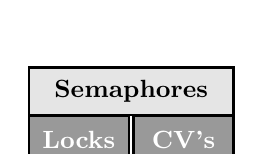
\begin{tikzpicture}[b/.style={draw, thick, minimum height=0.6cm, font=\small\bfseries, inner sep=3pt}]
  \node[b, fill=black!10, minimum width=2.6cm] at (0,0.62) {Semaphores};
  \node[b, fill=black!40, text=white, minimum width=1.27cm] at (-0.665,0) {Locks};
  \node[b, fill=black!40, text=white, minimum width=1.27cm] at (0.665,0) {CV's};
\end{tikzpicture}
\end{center}
(Top layer built on the bottom layer.) In the slides, \texttt{Sem\_wait()}
means ``decrement value, wait until value \(> 0\)''; \texttt{Sem\_post()}
means ``increment value, then wake a single waiter''.

\subsection{Build a lock from a semaphore}

\begin{lstlisting}
typedef struct __lock_t {
  sem_t sem;
} lock_t;

void init(lock_t *lock) {
  sem_init(&lock->sem, 1);   // 1 -> 1 thread can grab lock
}
void acquire(lock_t *lock) {
  sem_wait(&lock->sem);
}
void release(lock_t *lock) {
  sem_post(&lock->sem);
}
\end{lstlisting}

The slide first leaves the initial value as \texttt{??}; the answer is
\textbf{1}: one thread can grab the lock. The first \texttt{sem\_wait}
takes it to 0 and continues; a second caller takes it to \(-1\) and sleeps;
\texttt{release} posts and wakes it. A semaphore used this way is called a
\textbf{binary semaphore}.

\subsection{Build CVs over semaphores}

Possible, but \textbf{really hard to do right}. (The slide refers to
Microsoft Research's attempts: ``Implementing Condition Variables with
Semaphores'', \url{http://research.microsoft.com/pubs/64242/ImplementingCVs.pdf}.)

\keepspace{20\baselineskip}
\subsection{Build a semaphore from a lock and a CV}

The slides fill this in step by step: first the struct and init, then the
skeleton of wait/post (``this stuff is atomic'' between acquire and
release), then the bodies.

\begin{lstlisting}
typedef struct {
   int value;
   cond_t cond;
   lock_t lock;
} sem_t;

void sem_init(sem_t *s, int value) {
  s->value = value;
  cond_init(&s->cond);
  lock_init(&s->lock);
}

void sem_wait(sem_t *s) {
  lock_acquire(&s->lock);
  while (s->value <= 0)
     cond_wait(&s->cond);
  s->value--;
  lock_release(&s->lock);
}

void sem_post(sem_t *s) {
  lock_acquire(&s->lock);
  s->value++;
  cond_signal(&s->cond);
  lock_release(&s->lock);
}
\end{lstlisting}

\begin{itemize}
  \item \texttt{value} is the state; the lock makes each operation atomic;
        the CV is where waiters sleep.
  \item \texttt{sem\_wait} uses \texttt{while} (rule of thumb 3), and
        decrements only once the value is positive. So in this version the
        value never goes negative; it does not count waiters (the
        definition above allows that, but this implementation does not need
        it).
  \item (\texttt{cond\_wait} is written with one argument on the slide; it
        is waiting on \texttt{s->cond} with \texttt{s->lock}.)
\end{itemize}

\keepspace{28\baselineskip}
% ===========================================================================
\section{Producer/consumer with semaphores}
% ===========================================================================

\subsection{\#1: single producer, single consumer, single buffer}

\textbf{Requirements:}
\begin{itemize}
  \item the consumer must wait for the producer to fill the buffer;
  \item the producer must wait for the consumer to empty the buffer (if
        filled).
\end{itemize}
This requires 2 semaphores:
\begin{itemize}
  \item \texttt{emptyBuffer}: initialize to \textbf{1} \(\to\) 1 empty
        buffer; the producer can run 1 time first.
  \item \texttt{fullBuffer}: initialize to \textbf{0} \(\to\) 0 full
        buffers; the consumer can run 0 times first.
\end{itemize}

\begin{center}
\begin{minipage}[t]{0.47\textwidth}
\textbf{Producer}
\begin{lstlisting}[numbers=none]
while (1) {
  sem_wait(&emptyBuffer);
  Fill(&buffer);
  sem_signal(&fullBuffer);
}
\end{lstlisting}
\end{minipage}\hfill
\begin{minipage}[t]{0.47\textwidth}
\textbf{Consumer}
\begin{lstlisting}[numbers=none]
while (1) {
  sem_wait(&fullBuffer);
  Use(&buffer);
  sem_signal(&emptyBuffer);
}
\end{lstlisting}
\end{minipage}
\end{center}
(\texttt{sem\_signal} on these slides = \texttt{sem\_post}.)

\subsection{\#2: circular buffer, single producer, single consumer}

Shared buffer with \(N\) elements. Again 2 semaphores:
\begin{itemize}
  \item \texttt{emptyBuffer}: initialize to \textbf{\(N\)} \(\to\) \(N\)
        empty buffers; the producer can run \(N\) times first.
  \item \texttt{fullBuffer}: initialize to \textbf{0} \(\to\) 0 full
        buffers; the consumer can run 0 times first.
\end{itemize}

\begin{center}
\begin{minipage}[t]{0.47\textwidth}
\textbf{Producer}
\begin{lstlisting}[numbers=none]
i = 0;
while (1) {
  sem_wait(&emptyBuffer);
  Fill(&buffer[i]);
  i = (i+1)%N;
  sem_signal(&fullBuffer);
}
\end{lstlisting}
\end{minipage}\hfill
\begin{minipage}[t]{0.47\textwidth}
\textbf{Consumer}
\begin{lstlisting}[numbers=none]
j = 0;
while (1) {
  sem_wait(&fullBuffer);
  Use(&buffer[j]);
  j = (j+1)%N;
  sem_signal(&emptyBuffer);
}
\end{lstlisting}
\end{minipage}
\end{center}

The semaphore values count resources: \texttt{emptyBuffer} = number of empty
slots, \texttt{fullBuffer} = number of full slots. No lock is needed: with
one producer and one consumer, \texttt{i} is touched only by the producer
and \texttt{j} only by the consumer, and the semaphores keep them from
working on the same slot.

\keepspace{16\baselineskip}
\subsection{\#3: multiple producers, multiple consumers}

\textbf{Requirements:}
\begin{itemize}
  \item each consumer must grab a \textbf{unique filled} element;
  \item each producer must grab a \textbf{unique empty} element.
\end{itemize}

\begin{quizbox}[Why will the previous code not work? Are \texttt{i} and \texttt{j} private or shared?]
If \texttt{i} is private (one per producer), two producers both start at
slot 0 and fill the \emph{same} slot. If \texttt{i} is shared, the update
\texttt{i = (i+1)\%N} and the \texttt{Fill} race exactly like the shared
counter of Lecture 16. Either way, we need each producer to grab a unique
buffer (and likewise for consumers).
\end{quizbox}

The slides switch to finding a slot explicitly:

\begin{center}
\begin{minipage}[t]{0.47\textwidth}
\textbf{Producer}
\begin{lstlisting}[numbers=none]
while (1) {
  sem_wait(&emptyBuffer);
  myi = findempty(&buffer);
  Fill(&buffer[myi]);
  sem_signal(&fullBuffer);
}
\end{lstlisting}
\end{minipage}\hfill
\begin{minipage}[t]{0.47\textwidth}
\textbf{Consumer}
\begin{lstlisting}[numbers=none]
while (1) {
  sem_wait(&fullBuffer);
  myj = findfull(&buffer);
  Use(&buffer[myj]);
  sem_signal(&emptyBuffer);
}
\end{lstlisting}
\end{minipage}
\end{center}

\begin{quizbox}[Are \texttt{myi} and \texttt{myj} private or shared? Where is mutual exclusion needed?]
\texttt{myi}, \texttt{myj} are \textbf{private} (local to each thread). But
\texttt{findempty}/\texttt{findfull} inspect and claim slots of the
\emph{shared} buffer, so two producers could find the same empty slot.
Mutual exclusion is needed around finding (and claiming) a slot. Use a
semaphore \texttt{mutex} initialized to 1 as a lock.
\end{quizbox}

\keepspace{20\baselineskip}
\subsection{Three possible locations for mutual exclusion: which work, which is best?}

\begin{solbox}[Option \#1: mutex around everything --- deadlock]
\begin{center}
\begin{minipage}[t]{0.46\textwidth}
\begin{lstlisting}[numbers=none]
sem_wait(&mutex);
sem_wait(&emptyBuffer);
myi = findempty(&buffer);
Fill(&buffer[myi]);
sem_signal(&fullBuffer);
sem_signal(&mutex);
\end{lstlisting}
\end{minipage}\hfill
\begin{minipage}[t]{0.46\textwidth}
\begin{lstlisting}[numbers=none]
sem_wait(&mutex);
sem_wait(&fullBuffer);
myj = findfull(&buffer);
Use(&buffer[myj]);
sem_signal(&emptyBuffer);
sem_signal(&mutex);
\end{lstlisting}
\end{minipage}
\end{center}
\textbf{Problem: deadlock at mutex.} E.g.\ the consumer runs first: it takes
\texttt{mutex}, then sleeps on \texttt{fullBuffer} (nothing produced)
\emph{while still holding \texttt{mutex}}. The producer blocks on
\texttt{mutex} and can never produce. The consumer won't release the mutex.
\end{solbox}

\begin{solbox}[Option \#2: mutex inside the resource wait --- works, but limits concurrency]
\begin{center}
\begin{minipage}[t]{0.46\textwidth}
\begin{lstlisting}[numbers=none]
sem_wait(&emptyBuffer);
sem_wait(&mutex);
myi = findempty(&buffer);
Fill(&buffer[myi]);
sem_signal(&mutex);
sem_signal(&fullBuffer);
\end{lstlisting}
\end{minipage}\hfill
\begin{minipage}[t]{0.46\textwidth}
\begin{lstlisting}[numbers=none]
sem_wait(&fullBuffer);
sem_wait(&mutex);
myj = findfull(&buffer);
Use(&buffer[myj]);
sem_signal(&mutex);
sem_signal(&emptyBuffer);
\end{lstlisting}
\end{minipage}
\end{center}
A thread only takes \texttt{mutex} once it knows a slot is available, so it
never sleeps holding it. \textbf{Works, but limits concurrency}: only 1
thread at a time can be using or filling \emph{different} buffers.
\end{solbox}

\begin{solbox}[Option \#3: mutex only around finding a slot --- works and is best]
\begin{center}
\begin{minipage}[t]{0.46\textwidth}
\begin{lstlisting}[numbers=none]
sem_wait(&emptyBuffer);
sem_wait(&mutex);
myi = findempty(&buffer);
sem_signal(&mutex);
Fill(&buffer[myi]);
sem_signal(&fullBuffer);
\end{lstlisting}
\end{minipage}\hfill
\begin{minipage}[t]{0.46\textwidth}
\begin{lstlisting}[numbers=none]
sem_wait(&fullBuffer);
sem_wait(&mutex);
myj = findfull(&buffer);
sem_signal(&mutex);
Use(&buffer[myj]);
sem_signal(&emptyBuffer);
\end{lstlisting}
\end{minipage}
\end{center}
\textbf{Works and increases concurrency}: only finding a buffer is
protected by the mutex; filling or using \emph{different} buffers can
proceed concurrently. (\texttt{findempty}/\texttt{findfull} must mark the
slot as taken, so another thread does not find it before it is filled or
used.)
\end{solbox}

\keepspace{30\baselineskip}
% ===========================================================================
\section{Reader/writer locks}
% ===========================================================================

\begin{defbox}[Goal]
\begin{itemize}
  \item Let \textbf{multiple reader} threads grab the lock (\textbf{shared}).
  \item Only \textbf{one writer} thread can grab the lock
        (\textbf{exclusive}): no reader threads, no other writer threads.
\end{itemize}
\end{defbox}

\begin{lstlisting}
typedef struct _rwlock_t {
   sem_t lock;      // binary semaphore (basic lock)
   sem_t writelock; // used to allow ONE writer or MANY readers
   int readers;     // count of readers reading in critical section
} rwlock_t;

void rwlock_init(rwlock_t *rw) {
   rw->readers = 0;
   sem_init(&rw->lock, 1);
   sem_init(&rw->writelock, 1);
}

void rwlock_acquire_readlock(rwlock_t *rw) {
    sem_wait(&rw->lock);
    rw->readers++;
    if (rw->readers == 1) // first reader acquires writelock
        sem_wait(&rw->writelock);
    sem_post(&rw->lock);
}

void rwlock_release_readlock(rwlock_t *rw) {
    sem_wait(&rw->lock);
    rw->readers--;
    if (rw->readers == 0) // last reader releases writelock
        sem_post(&rw->writelock);
    sem_post(&rw->lock);
}

rwlock_acquire_writelock(rwlock_t *rw) { sem_wait(&rw->writelock); }
rwlock_release_writelock(rwlock_t *rw) { sem_post(&rw->writelock); }
\end{lstlisting}

The slides highlight the code in three passes:
\begin{enumerate}
  \item \textbf{\texttt{lock} (binary semaphore):} the
        \texttt{sem\_wait(\&rw->lock)} / \texttt{sem\_post(\&rw->lock)} pairs
        just protect the shared counter \texttt{readers}, like any lock.
  \item \textbf{First reader in:} when \texttt{readers} becomes 1, that
        reader acquires \texttt{writelock} on behalf of \emph{all} readers.
        Later readers just increment the count and enter. A writer waiting
        on \texttt{writelock} is shut out.
  \item \textbf{Last reader out:} when \texttt{readers} drops to 0, that
        reader releases \texttt{writelock}, letting a writer in.
\end{enumerate}
A writer simply takes \texttt{writelock}, so it excludes other writers and
(since the first reader also needs \texttt{writelock}) all readers.

\begin{warnbox}[Fairness problem]
\begin{itemize}
  \item It would be relatively easy for \textbf{readers to starve a
        writer}: as long as at least one reader is inside, new readers keep
        entering, and \texttt{readers} never reaches 0.
  \item How to prevent more readers from entering the lock once a writer is
        waiting? (Left as an open question on the slide.)
\end{itemize}
\end{warnbox}

% ===========================================================================
\section{The dining philosophers}
% ===========================================================================

\begin{itemize}
  \item Assume there are \textbf{five ``philosophers''} sitting around a
        table.
  \item Between each pair of philosophers is a \textbf{single fork} (five
        total).
  \item The philosophers each have times where they \textbf{think}, and
        don't need any forks, and times where they \textbf{eat}.
  \item In order to eat, a philosopher needs \textbf{two forks}, both the
        one on their left and the one on their right.
  \item There is contention for these forks.
\end{itemize}

\begin{center}
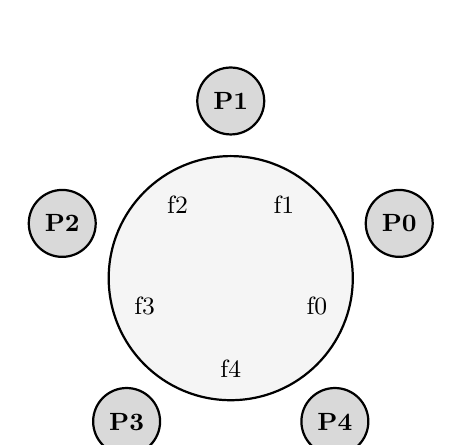
\begin{tikzpicture}[ph/.style={circle, draw, thick, fill=black!15, minimum size=0.85cm, font=\small\bfseries},
  fk/.style={font=\small}]
  \draw[thick, fill=black!4] (0,0) circle (1.55);
  \foreach \i/\ang in {1/90, 0/18, 4/-54, 3/-126, 2/162} {
    \node[ph] at (\ang:2.25) {P\i};
  }
  \foreach \i/\ang in {1/54, 0/-18, 4/-90, 3/-162, 2/126} {
    \node[fk] at (\ang:1.15) {f\i};
  }
\end{tikzpicture}
\end{center}

Philosopher \(p\) sits between fork \(p\) (left) and fork \((p+1) \bmod 5\)
(right); e.g.\ P0 is between f0 and f1, P4 between f4 and f0.

\begin{keybox}[Key challenge]
\begin{itemize}
  \item There is \textbf{no deadlock}.
  \item \textbf{No philosopher starves} and never gets to eat.
  \item \textbf{Concurrency is high}.
\end{itemize}
\end{keybox}

\begin{center}
\begin{minipage}[t]{0.42\textwidth}
\textbf{Basic loop of each philosopher}
\begin{lstlisting}[numbers=none]
while (1) {
   think();
   getforks();
   eat();
   putforks();
}
\end{lstlisting}
\end{minipage}\hfill
\begin{minipage}[t]{0.52\textwidth}
\textbf{Helper functions (Downey's solutions)}
\begin{lstlisting}[numbers=none]
int left(int p)  { return p; }
int right(int p) { return (p + 1) % 5; }
\end{lstlisting}
\end{minipage}
\end{center}
Philosopher \(p\) refers to the fork on their left by calling
\texttt{left(p)}, and to the fork on their right by calling
\texttt{right(p)}.

\keepspace{16\baselineskip}
\subsection{Broken solution: one semaphore per fork}

We need some semaphores, one for each fork: \texttt{sem\_t forks[5]} (each
initialized to 1).

\begin{lstlisting}
void getforks() {
   sem_wait(forks[left(p)]);
   sem_wait(forks[right(p)]);
}

void putforks() {
   sem_post(forks[left(p)]);
   sem_post(forks[right(p)]);
}
\end{lstlisting}

\begin{warnbox}[Deadlock occurs!]
If each philosopher happens to grab the fork on their \textbf{left} before
any philosopher can grab the fork on their right, each will be stuck holding
one fork and waiting for another, \textbf{forever}. (P0 holds f0 and waits
for f1, held by P1, who waits for f2, \ldots, P4 holds f4 and waits for f0,
held by P0: a cycle.)
\end{warnbox}

\subsection{A solution: breaking the dependency}

Change how forks are acquired: let philosopher 4 acquire the forks in a
\textbf{different order}.

\begin{lstlisting}
void getforks() {
   if (p == 4) {
      sem_wait(forks[right(p)]);
      sem_wait(forks[left(p)]);
   } else {
      sem_wait(forks[left(p)]);
      sem_wait(forks[right(p)]);
   }
}
\end{lstlisting}

There is no situation where each philosopher grabs one fork and is stuck
waiting for another: \textbf{the cycle of waiting is broken}. P4 first
tries f0 (its right fork). If everyone else has taken their left fork, P0
holds f0, so P4 waits \emph{without} holding f4, and P3 can take f4, eat,
and release; the chain unwinds.

\keepspace{22\baselineskip}
% ===========================================================================
\section{Summary}
% ===========================================================================

\begin{keybox}[Semaphores]
\begin{itemize}
  \item Semaphores are \textbf{equivalent to locks + condition variables}:
        they can be used for both \textbf{mutual exclusion} and
        \textbf{ordering}.
  \item Semaphores \textbf{contain state}; how they are initialized depends
        on how they will be used:
    \begin{itemize}
      \item \textbf{init to 1}: mutex;
      \item \textbf{init to 0}: join (1 thread must arrive first, then the
            other);
      \item \textbf{init to \(N\)}: number of available resources.
    \end{itemize}
  \item \texttt{sem\_wait()}: waits until value \(> 0\), then decrements
        (atomic).
  \item \texttt{sem\_post()}: increments the value, then wakes a single
        waiter (atomic).
  \item Semaphores can be used in \textbf{producer/consumer} relationships
        and for \textbf{reader/writer locks}.
\end{itemize}
\end{keybox}

\begin{center}
\renewcommand{\arraystretch}{1.18}
\small
\begin{tabularx}{\textwidth}{@{}lX@{}}
  \toprule
  \textbf{Use} & \textbf{Semaphores and initial values} \\
  \midrule
  Lock & one semaphore, init 1 \\
  Join & one semaphore, init 0; parent waits, child posts \\
  P/C, 1 slot & \texttt{emptyBuffer} = 1, \texttt{fullBuffer} = 0 \\
  P/C, \(N\) slots & \texttt{emptyBuffer} = \(N\), \texttt{fullBuffer} = 0 \\
  P/C, many threads & as above + \texttt{mutex} = 1 around \texttt{findempty}/\texttt{findfull} only \\
  Reader/writer lock & \texttt{lock} = 1 (protects \texttt{readers}), \texttt{writelock} = 1 \\
  Dining philosophers & \texttt{forks[5]} = 1 each; one philosopher picks up in reverse order \\
  \bottomrule
\end{tabularx}
\end{center}

\end{document}
